\documentclass[12pt]{article}

\usepackage{amssymb,amsmath,amsfonts,bbm,bm,dcolumn,booktabs,eurosym,geometry,ulem,graphicx,color,xcolor,setspace,sectsty,comment,float,caption,subfigure,array,hyperref}
\usepackage{xurl}
\usepackage[font=bf]{caption}
\usepackage[bottom]{footmisc}

\hypersetup{
    colorlinks,
    linkcolor={black},
    citecolor={blue!35!black},
    urlcolor={blue!35!black}
}

\geometry{left=1.0in,right=1.0in,top=1.0in,bottom=1.0in}

\begin{document}
\title{Development Economics Problem Set 2}
\author{Steven VanOmmeren\thanks{A complete replication package of this project is available at \url{https://github.com/svanomm/development-econ/}.}}
\date{\today}
\maketitle

\doublespacing
\noindent
Before answering the questions, please note my data preparation steps. I use 2016 data where available and 2015 data to fill in any missing values. I also reviewed the full list of country codes, and I removed any codes that refer to groups of countries, leaving only the individual countries in the dataset.\footnote{Full list of country codes that I dropped: ARB,CSS,CEB,EAR,EAS,TEA,EAP,ECS,TEC,ECA,EUU,\\ FCS,HPC,HIC,IBD,IBT,IDB,DFS,IDX,IDA,LTE,LCN,LAC,TLA,LDC,LMY,LIC,LMC,MEA,TMN,\\ MNA,MIC,NAC,OED,OSS,PSS,PST,PRE,SST,SAS,TSA,SSF,TSS,SSA,UMC,WLD.} Some of the variables that I analyze below are missing for certain countries. In this case, those countries are excluded from the analysis. I also used the Top 20\% and Bottom 20\% variables to create a Top-Bottom Quintile Ratio variable, which I use as an additional measure of income inequality.

\begin{enumerate}
    \item \textbf{For the key variables of interest – poverty, income, and inequality - report a table of summary statistics – Mean, Median, Min, Max, Std. Dev., 25th percentile and coefficient of variation.}
    
    \begin{figure}[H]
        \centering
        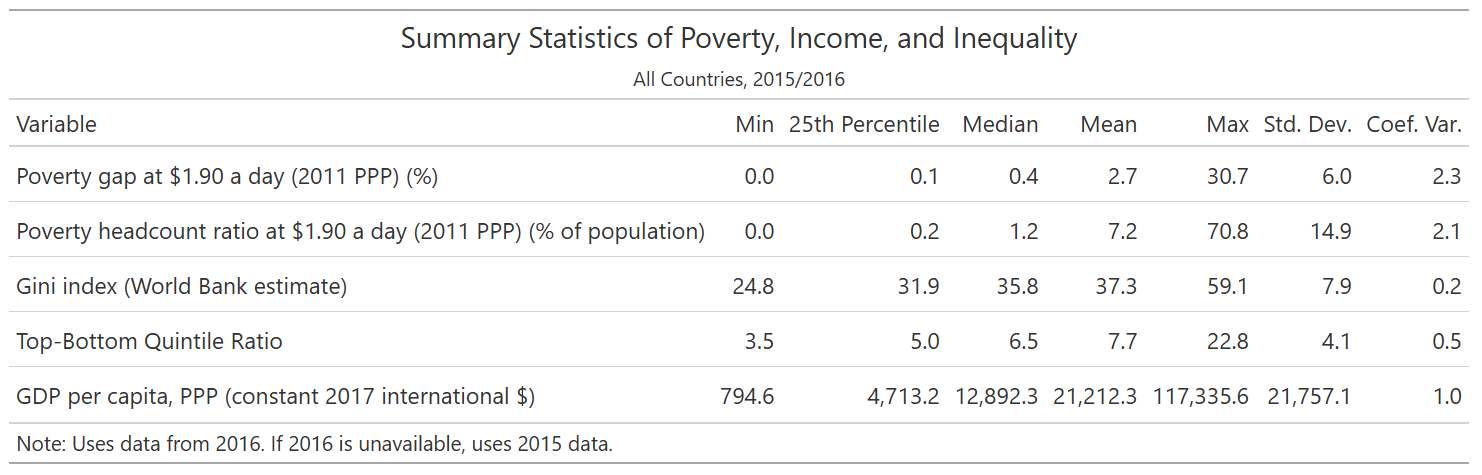
\includegraphics[width=\textwidth]{./output/summary_stats_table.png}
    \end{figure}

    \begin{enumerate}
        \singlespace
        \item \textbf{What is the average income inequality?}
        \\\\
        I measured income inequality two ways, the Gini index and the ratio of top quintile to bottom quintile share of income. The average Gini index is 37.3 in my sample, while the average ratio of top-bottom quintile ratio is 7.7.

        \item \textbf{Create a dummy variable to divide countries into three different income groups. What proportion of the sample is rich/poor?}
        \\\\
        I created a dummy variable that divides countries into three income groups: low income, middle income, and high income. Because I did not have a prior on where the splits should be, I made them equally spaced. So, one-third of the countries are considered poor and one-third are considered rich. However, if you then look at the population within each group, only 19\% of the population lives within those high-income countries, while the lower- and middle-income countries have about 40\% each.

        \item \textbf{What is the average inequality for the rich countries?}
        \\\\
        In my data, the rich countries have an average Gini index of 32.9, while the top-bottom quintile ratio is 5.9.

        \item \textbf{Find a cross tabulation of inequality and poverty by income group?}
        \\\\
        My cross-tabulation shows that inequality is highest for middle-income countries, though poor countries have a very similar Gini index and Top-Bottom Quintile Ratio. Conversely, inequality is noticeably lower in high-income countries.
        \begin{figure}[H]
            \centering
            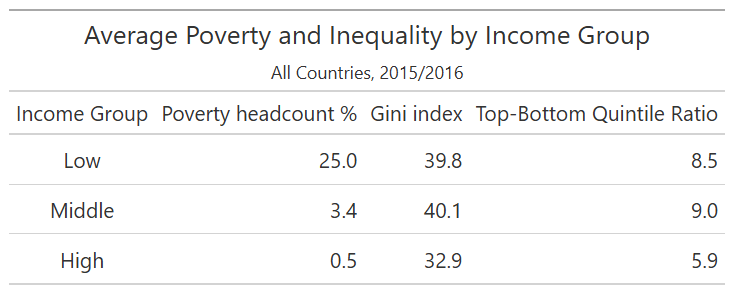
\includegraphics[width=0.8\textwidth]{./output/inequality_poverty_table.png}
        \end{figure}

    \end{enumerate}
    \item \textbf{What is the correlation between inequality, poverty, and income?}
    \\\\
    My correlation matrix shows that inequality and poverty are positively correlated, with a correlation coefficient of 0.42 or 0.37 (depending on which inequality measure is used). Inequality and income are negatively correlated, with a coefficient of -0.40 or -0.32. Poverty and income are negatively correlated, with a coefficient of -0.43.
    \begin{figure}[H]
        \centering
        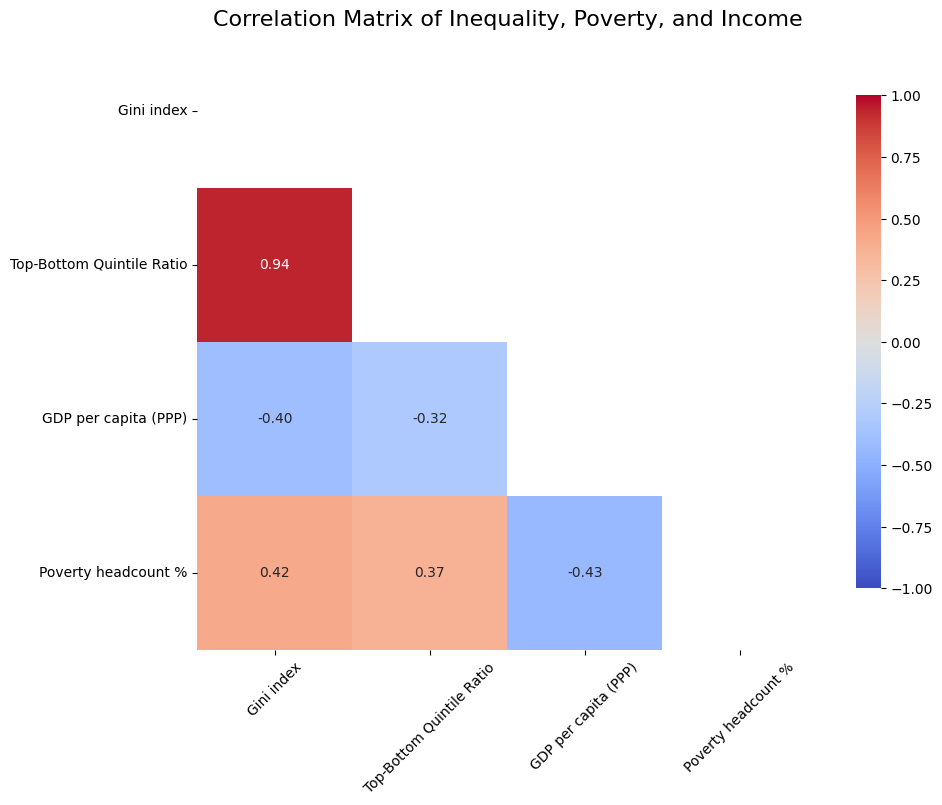
\includegraphics[width=0.8\textwidth]{./output/correlation_matrix.png}
    \end{figure}
    \item \textbf{What is the interquartile range for inequality? What is the variance in inequality? Do inequality and other variables co-vary?}
    \\\\
    In my data, the interquartile range for the Gini index is 10.5 and for the Top-Bottom Quintile Ratio is 3.7. The variance in the Gini index is 62.8 and for the Top-Bottom Quintile Ratio is 16.4. Inequality covaries with income and poverty, as demonstrated by the correlation matrix above.
    \item \textbf{Provide the five-number summary for inequality, poverty, and income, for the middle income countries only.}
    \begin{figure}[H]
        \centering
        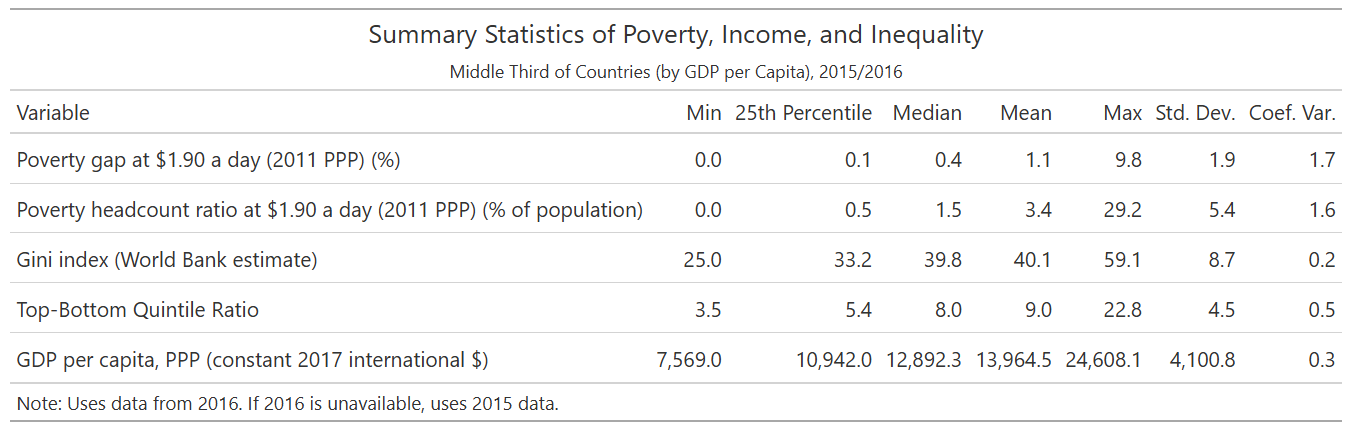
\includegraphics[width=\textwidth]{./output/summary_stats_table_middle_income.PNG}
    \end{figure}
    \item \textbf{Plot a scatterplot of poverty and inequality. Include a line of fit.}
    \\\\
    The scatter plot is hard to figure out what relationship is showing because the poverty headcount percent is bunched around zero. The line of fit shows a positive relationship between inequality and poverty, but the line is clearly not fitting very well.

    \begin{figure}[H]
        \centering
        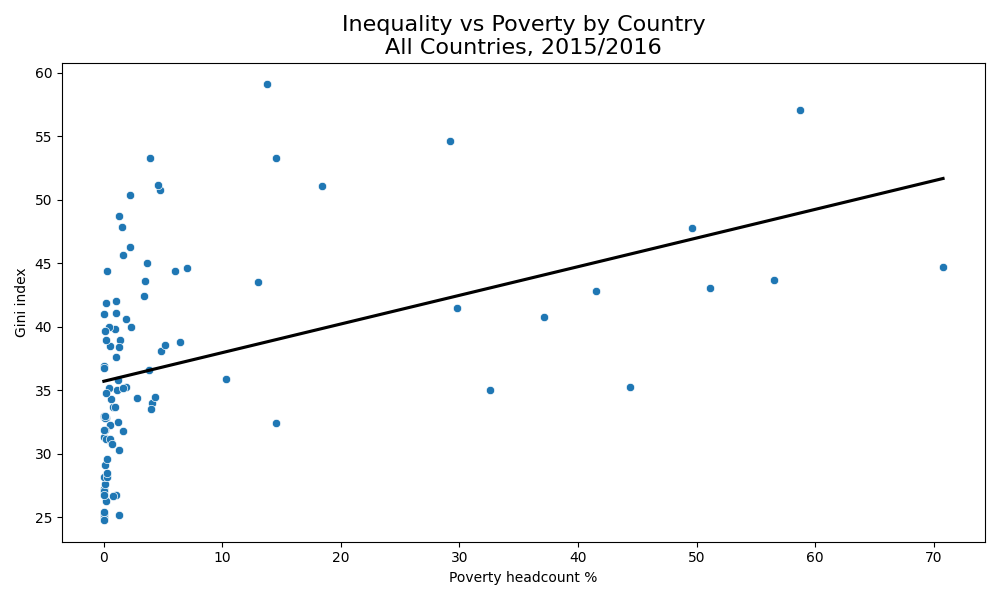
\includegraphics[width=0.8\textwidth]{./output/Scatterplot Inequality vs Poverty.png}
    \end{figure}
    \item \textbf{Now you are ready to run the regressions - Regress and interpret the effect of (a) income on poverty; (b) income on inequality; and (c) inequality on poverty.}
    \\\\
    \textbf{Income (GDP per capita, PPP) on Poverty headcount \%:}
    \footnotesize
    \begin{center}
\begin{tabular}{lcccccc}
\toprule
                                    & \textbf{coef} & \textbf{std err} & \textbf{t} & \textbf{P$> |$t$|$} & \textbf{[0.025} & \textbf{0.975]}  \\
\midrule
\textbf{const}                      &      14.5654  &        2.090     &     6.971  &         0.000        &       10.417    &       18.714     \\
\textbf{GDP per capita, PPP (\$Ks)} &      -0.3258  &        0.070     &    -4.656  &         0.000        &       -0.465    &       -0.187     \\
\bottomrule
\end{tabular}
\end{center}
    \normalsize
    This regression shows that a \$1,000 PPP increase in GDP per capita is associated with a -0.33 percentage point decrease in poverty headcount \%, i.e. richer countries tend to have lower poverty rates. The regression predicts that to completely eliminate poverty, a country would need a GDP per capita of at least \$44,707 PPP.
    \\\\
    \textbf{Income (GDP per capita, PPP) on Inequality (Gini index):}
    \footnotesize
    \begin{center}
\begin{tabular}{lcccccc}
\toprule
                                    & \textbf{coef} & \textbf{std err} & \textbf{t} & \textbf{P$> |$t$|$} & \textbf{[0.025} & \textbf{0.975]}  \\
\midrule
\textbf{const}                      &      40.9519  &        1.134     &    36.099  &         0.000        &       38.700    &       43.204     \\
\textbf{GDP per capita, PPP (\$Ks)} &      -0.1597  &        0.038     &    -4.204  &         0.000        &       -0.235    &       -0.084     \\
\bottomrule
\end{tabular}
\end{center}
    \normalsize
    This regression shows that a \$1,000 PPP increase in GDP per capita is associated with a -0.16 percentage point decrease in the Gini index, i.e. richer countries tend to have lower income inequality. The regression predicts that to completely eliminate income inequality (Gini index of 0), a country would need a GDP per capita of \$256,430 PPP.
    \\\\
    \textbf{Inequality (Gini index) on Poverty headcount \%:}
    \footnotesize
    \begin{center}
\begin{tabular}{lcccccc}
\toprule
                    & \textbf{coef} & \textbf{std err} & \textbf{t} & \textbf{P$> |$t$|$} & \textbf{[0.025} & \textbf{0.975]}  \\
\midrule
\textbf{const}      &     -22.3784  &        6.652     &    -3.364  &         0.001        &      -35.585    &       -9.172     \\
\textbf{Gini index} &       0.7923  &        0.174     &     4.546  &         0.000        &        0.446    &        1.138     \\
\bottomrule
\end{tabular}
\end{center}
    \normalsize
    This regression shows that a 1 percentage point increase in the Gini index is associated with a 0.79 percentage point increase in poverty headcount \%, i.e. countries with higher income inequality tend to have higher poverty rates. The regression is clearly not designed for extreme-value predictions, as it would predict a poverty headcount \% of -22.4\% for a Gini index of 0 (perfect equality).

    \item \textbf{Instead of using income, use the dummy variables for whether the country is rich vs poor in your regression of income on poverty. Interpret the coefficients carefully.}
    \\\\
    \textbf{Income Group on Poverty headcount \%:}
    \footnotesize
    \begin{center}
\begin{tabular}{lcccccc}
\toprule
                            & \textbf{coef} & \textbf{std err} & \textbf{t} & \textbf{P$> |$t$|$} & \textbf{[0.025} & \textbf{0.975]}  \\
\midrule
\textbf{const}              &       3.3667  &        1.813     &     1.857  &         0.066        &       -0.233    &        6.967     \\
\textbf{Income Group\_Low}  &      21.6015  &        3.019     &     7.155  &         0.000        &       15.607    &       27.596     \\
\textbf{Income Group\_High} &      -2.8444  &        2.617     &    -1.087  &         0.280        &       -8.041    &        2.352     \\
\bottomrule
\end{tabular}
\end{center}
    \normalsize
    In this regression, I have omitted the category of middle-income countries to avoid collinearity. This means that the coefficients on the high and low categories are interpreted relative to middle-income countries. The coefficients indicate that rich countries have a 2.8 percentage point lower poverty headcount \% than middle-income countries, while poor countries have a 21.6 percentage point higher poverty headcount \% than middle-income countries. The constant indicates that the average poverty headcount \% in middle-income countries is 3.4\%. This regression demonstrates diminishing marginal returns to poverty rate as income increases, since high-income countries are not very different from middle-income countries, but poor countries are very different from middle-income countries in terms of poverty \%.


    \item \textbf{Do you expect any non-linearity in your regression, in which variable? Why? Test your hypothesis.}
    \\\\
    Yes, I would generally expect non-linear relationships between inequality, income, and poverty. One reason is from the Kuznets curve, which suggests that inequality increases with income at first, but then decreases as income continues to rise. I tested this hypothesis by running a regression of Gini index on GDP per capita and its square. The results disagree with Kuznets' hypothesis: the coefficient on GDP per capita is negative, while the coefficient on GDP per capita squared is positive (though not statistically significant).
    \\\\
    \textbf{Regression on Gini index:}
    \footnotesize
    \begin{center}
\begin{tabular}{lcccccc}
\toprule
                               & \textbf{coef} & \textbf{std err} & \textbf{t} & \textbf{P$> |$t$|$} & \textbf{[0.025} & \textbf{0.975]}  \\
\midrule
\textbf{const}                 &      42.3976  &        1.449     &    29.257  &         0.000        &       39.520    &       45.275     \\
\textbf{Income (\$Ks)}         &      -0.2927  &        0.092     &    -3.180  &         0.002        &       -0.475    &       -0.110     \\
\textbf{Income Squared (\$Ks)} &       0.0017  &        0.001     &     1.584  &         0.117        &       -0.000    &        0.004     \\
\bottomrule
\end{tabular}
\end{center}
    \normalsize
    As we saw in the scatter plot of inequality vs poverty above, poverty is generally bunched around zero, and the line of fit is clearly not linear. One way to test for non-linearity is by plotting Gini Index against log of poverty. It is clear from this scatter plot that the relationship is non-linear because the line of fit with log-poverty is much better. This relationship exhibits diminishing returns to inequality as poverty headcount ratio increases.
    \begin{figure}[H]
        \centering
        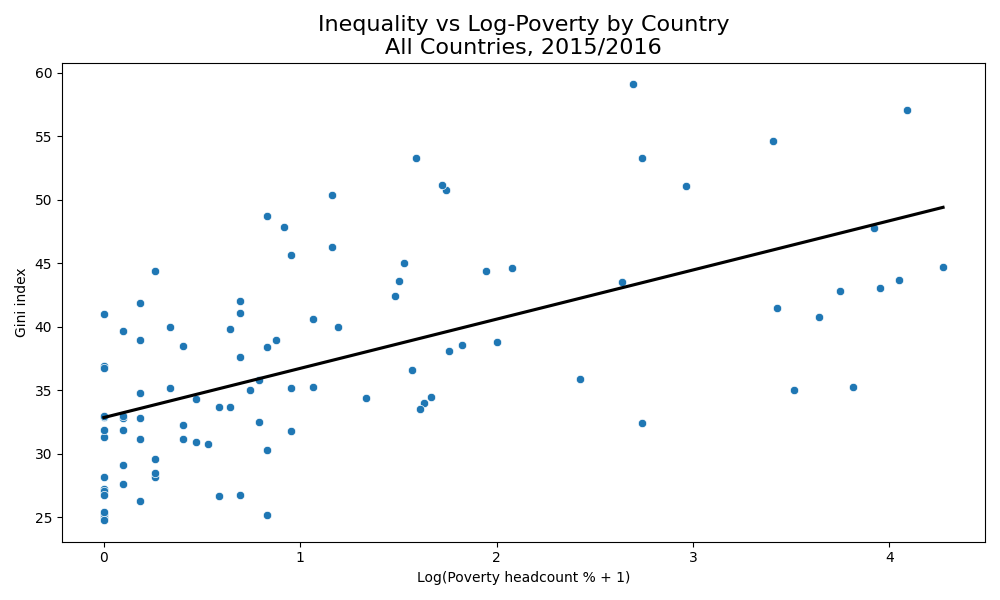
\includegraphics[width=0.8\textwidth]{./output/Scatterplot Inequality vs Log-Poverty.png}
    \end{figure}

    \item \textbf{Run diagnostic tests i.e. Are the error terms normal? Are they homoscedastic? Is there any evidence of autocorrelation, outliers, etc.?}
    \\\\
    I checked the residuals of two models: inequality (Gini index) on poverty, and inequality on log poverty. The plots below show that while neither models are perfect, the log-poverty model is preferred. This is because its residuals are closer to Normally-distributed, and the residiuals are more symmetric around zero. That being said, there is clear heteroskedasticity in both models, suggesting that robust standard errors are needed.
    
    \begin{figure}[H]
        \centering
        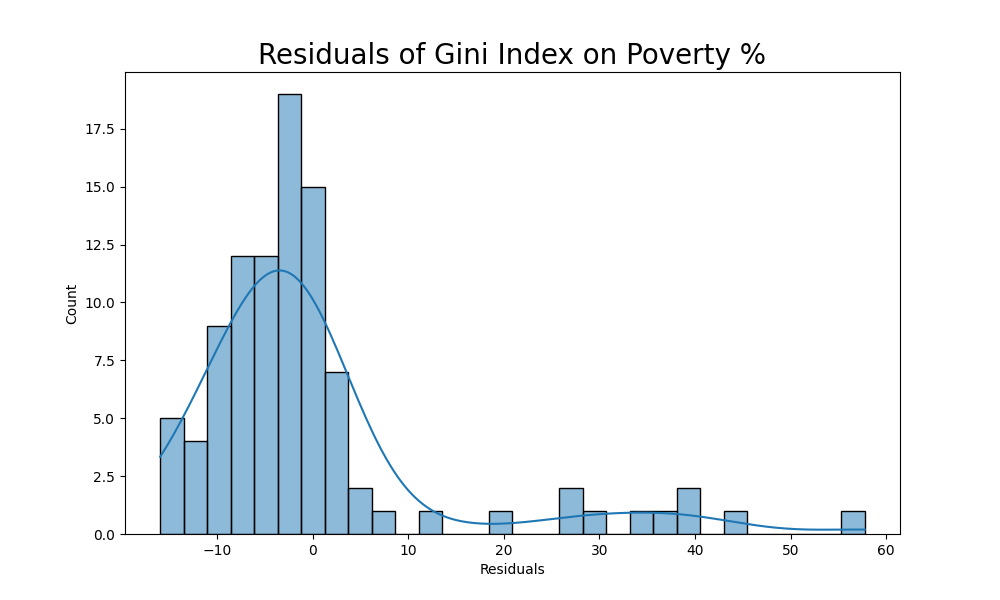
\includegraphics[width=0.45\textwidth]{./output/hist_inequality_poverty.png}
        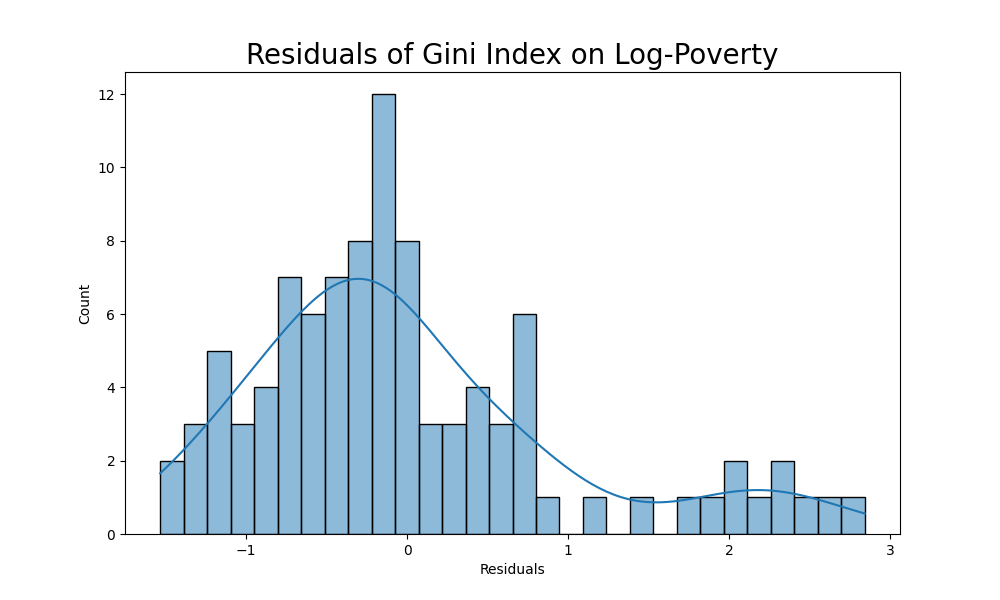
\includegraphics[width=0.45\textwidth]{./output/hist_inequality_log_poverty.png}
    \end{figure}
    
    \begin{figure}[H]
        \centering
        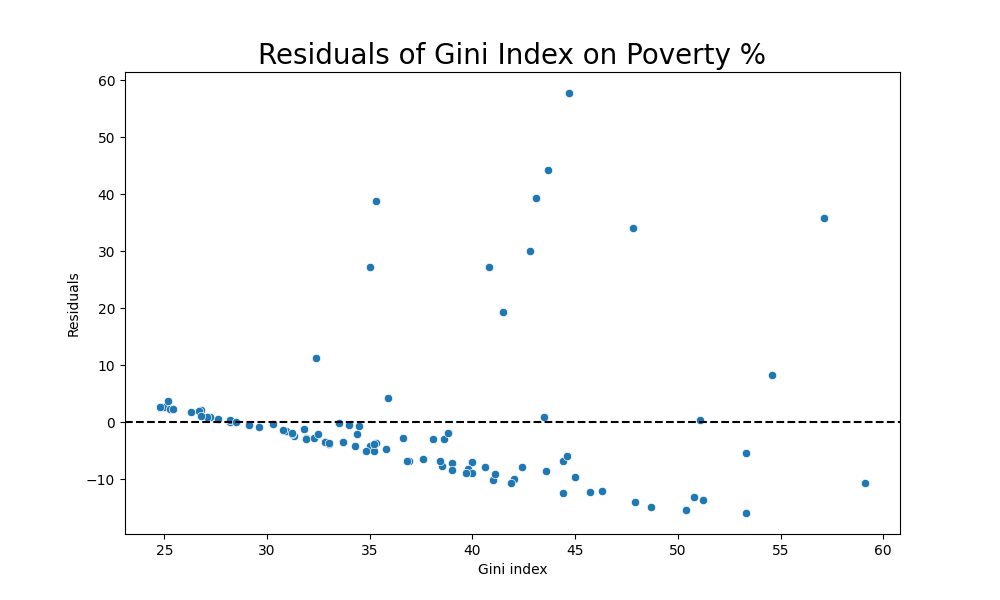
\includegraphics[width=0.45\textwidth]{./output/scatter_inequality_poverty.png}
        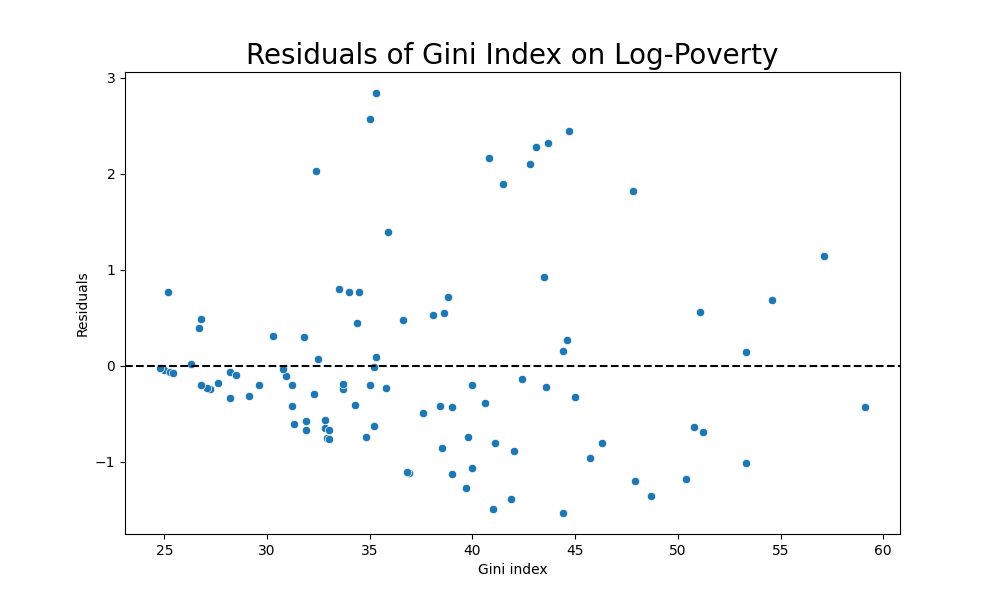
\includegraphics[width=0.45\textwidth]{./output/scatter_inequality_log_poverty.png}
    \end{figure}

    \item \textbf{Bonus: Anything else you like to do. (Don’t go overboard).}
    \\\\
    The Gini coefficient is not a perfect measure of inequality for a country, so it is important to look at multiple inequality metrics. This is why I created the top-bottom quintile ratio as an alternative measure. Looking at my correlation matrix, we can see that the two inequality measures are highly correlated with a correlation of 0.94. This suggests that, in my data set, the two can be used nearly interchangeably. Also, none of my conclusions change when using one metric versus the other.

    Below is a plot of the two inequality measures against each other. A smoothed line of fit shows a slightly non-linear relationship, though it is close to linear.
    \begin{figure}[H]
        \centering
        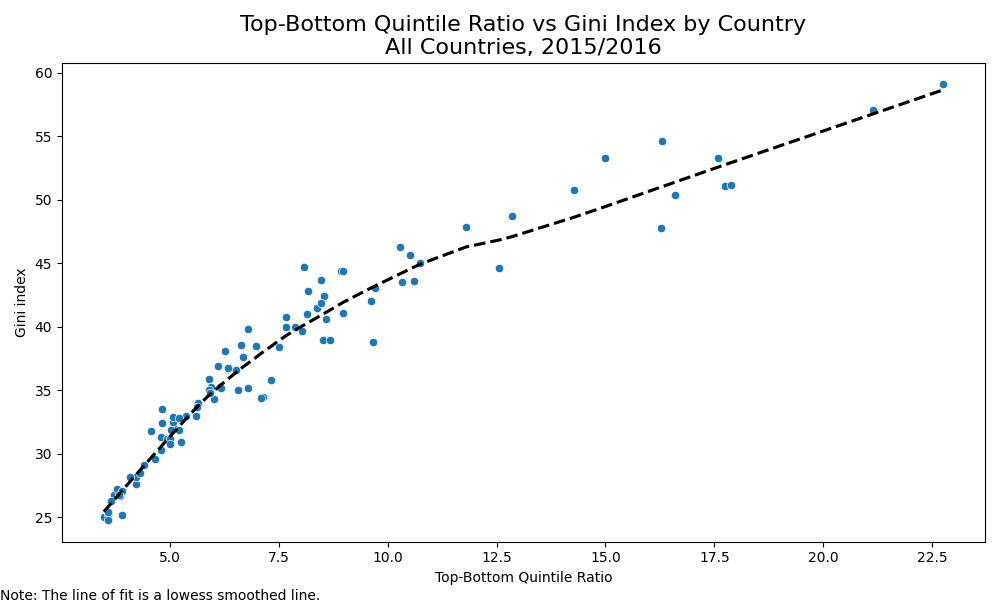
\includegraphics[width=0.8\textwidth]{./output/Scatterplot Top-Bottom Quintile Ratio vs Gini Index.png}
    \end{figure}
\end{enumerate}
\end{document}